\section{Método da Secante}
%\index{Método da Secante}

\subsection{Características}

\begin{itemize}
\item Necessita de duas aproximações iniciais da raiz desejada
\item Usa a reta secante passando por dois valores de $f$ consecutivos no processo iterativo.
\end{itemize}

\subsection{Descrição}

\begin{figure}[htb]
  %\index{figura da posição falsa modificado}%
  \setlength{\abovecaptionskip}{20pt}
  %%% o valor default de \abovecaptionskip definido para a classe
  %%% article e de 10pt.
  \centering
  %%% VIDE ABAIXO COMENTARIO SOBRE USO DE DIRETORIOS NO PATHNAME
  %%% DOS ARQUIVOS INCLUIDOS.
  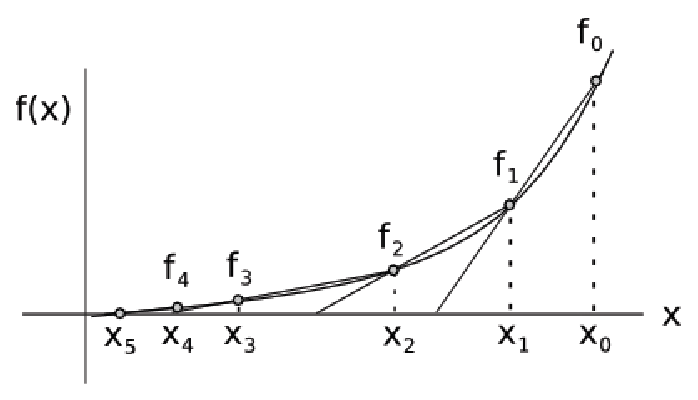
\includegraphics[scale=0.8]{capitulos/capitulo1/figuras/secante1.eps}
  \caption{Descrição do método da secante.}
  \label{fig:secante1}
\end{figure}

Considerando-se $h = x_{n-1} - x_{n-2}$ e utilizando-se \textit{backward} diferença finita para calcular $f'(x_{n-1})$ temos:

\[
 f'(x_{n-1}) = \frac{f(x_{n-1}) - f(x_{n-2})}{x_{n-1} - x_{n-2}}
\]

\[
 x_{n} = x_{n-1} - \frac{f(x_{n-1})}{f'(x_{n-1})} \approx x_{n-1} - \frac{f(x_{n-1})}{\frac{\displaystyle f(x_{n-1}) - f(x_{n-2})}{\displaystyle x_{n-1} - x_{n-2}}}
\]

\[
x_{n} = x_{n-1} - \frac{x_{n-1} - x_{n-2}}{f_{n-1} - f_{n-2}} \ast f_{n-1}
\]

\[
 n = 2, 3, ...
\]